\section{Numerical experiments}\label{sec:numerics}

In this section we verify numerically that the order of the constructed 
Runge-Kutta scheme $TM^{n-2}R$, for which $M$ is an SSPRK($s$,$q$,$p$) 
method, is indeed equal to the effective order $q$ of method $M$. 
For simplicity we call the $TM^{n-2}R$ scheme as \emph{ESSPRK-scheme}. 
A convergence study is performed on a smooth nonlinear ode problem. 
Also we show that the ESSP-scheme inherits the properties of the 
SSPRK($s,q,p$) method. 
In particular, the time-step restriction of the ESSPRK-scheme is the same 
with that of the main method $M$. 
This is demonstrated by showing the effect of the SSP coefficient on 
Burgers' equation.

\subsection{Convergence study}\label{subsec:convergence}
We consider the nonlinear equation
\begin{equation}\label{eq:conv_eq}
    u'(t) = -\frac{3}{2}u^{2}(t), \quad t \in [0,1], \quad \text{with } u(0) = 10,
\end{equation}
and exact solution
\begin{equation}\label{eq:conv_eq_exact}
    u(t) = 10/(15t + 1).
\end{equation}
We solve the initial value problem \eqref{eq:conv_eq} and 
\eqref{eq:conv_eq_exact} using an ESSPRK-scheme where $M$ is an 
ESSPRK($s,q,p$) method for $q = 3, 4$ and $p = 2$.
The stages of the permutation methods were kept as low as possible, thus 
we use two stages for a third-effective order method $M$ and four stages for 
a fourth-effective order method. 
The solution is computed for $N = 50.2^{k}$ for $k = 0, 1, 2, \dots, 6$ and 
hence the time-step used is $\Dt = \tfrac{1}{N} = \tfrac{2^{(1-k)}}{100}$ 
for each computation. 
The error between the exact solution and the approximation with respect 
to time-step is shown in Figure~\ref{fig:conv_study} on a logarithmic scale.
The convergence study was performed for various stages and the results 
show that the ESSPRK-scheme attends order equal to the effective order of 
method $M$. 
An important observation is that the error has order equal to the classical 
order of the main method and it is only increased when the finishing method 
is applied.
Finally, we note that for a fixed time-step increasing the number of stages
decreases the error.

\begin{figure}
	\centering
     \subfloat[SSPRK($s,3,2$)]{\label{fig:burgers_cont_a}
     \includegraphics[width=0.5\textwidth]{Pictures/convergence_3rd_ord}}
     \subfloat[SSPRK($s,4,2$)]{\label{fig:burgers_cont_b}
    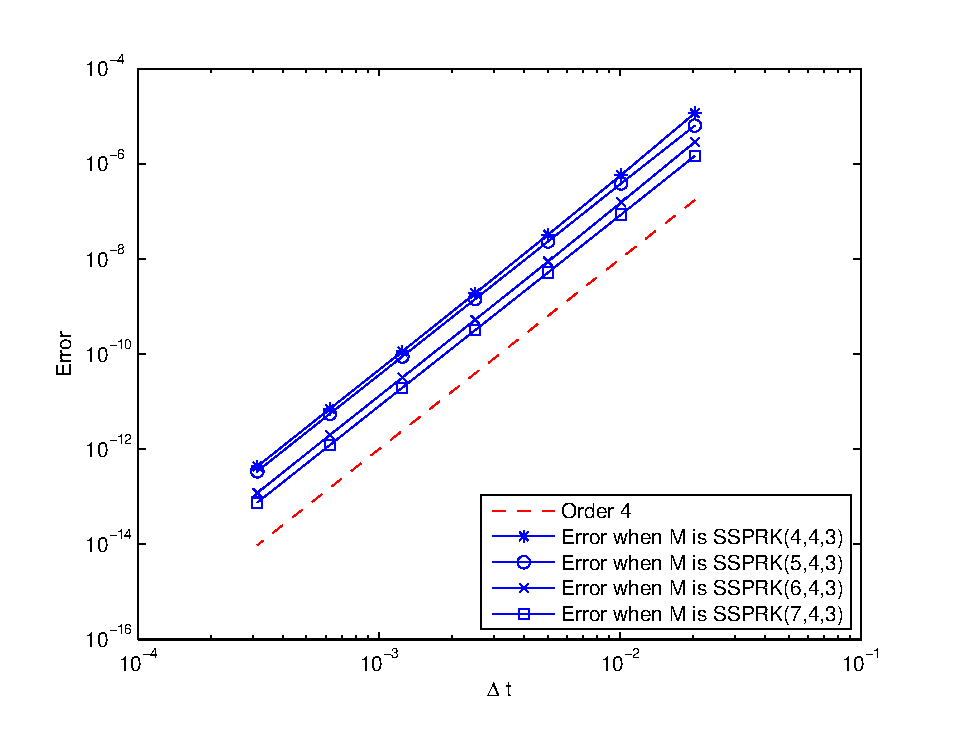
\includegraphics[width=0.5\textwidth]{Pictures/convergence_4th_ord_(2)}}
    \caption{Convergence of $TM^{n-2}R$ Runge-Kutta scheme when (a) $M$ 
    is an SSPRK($s,3,2$) method and (b) $ M $ is an SSPRK($s,4,2$) method.}
    \label{fig:conv_study}
\end{figure}

\subsection{Application to nonlinear problems}\label{subsec:nonlinear_problems}
\subsubsection{Burgers' equation}\label{subsubsec:burgers}
The inviscid Burgers' equation consists of the hyperbolic conservation law
\begin{equation}\label{eq:HCL}
    U_{t} + f(U)_{x} = 0,
\end{equation}
when the flux function $f(U) = \frac{1}{2}U^{2}$. 
We consider initial data
\begin{equation}\label{eq:burgers_IC}
    u(0,x)  = \frac{1}{2} - \frac{1}{4}sin{\pi x},
\end{equation}
on a periodic domain $x \in [0,2)$. 
The solution advances to the right where it eventually exhibits a shock. 
We perform a semi-discetisation of $f(U)_{x}$ using an upwind approximation 
\cite{Ketcheson2009} that gives
\begin{equation}\label{eq:burgers_flux}
    f(U)_{x} \approx \frac{1}{\Dt}\bigl(f(u_{i}) - f(u_{i-1})\bigr).
\end{equation}

The above time discretisation is SSP when coupled with Forward Euler method 
under time restriction $\Dt \leq {\Dt}_{FE} = \frac{\Delta x}{\|u(0,x)\|_{\infty}}$. 
We integrate to time $t_{f} = 2.3$ with $m = 256$ points in space.
\newline

\begin{figure}[t!]
    \centering
    \subfloat[$\sigma = $]{\label{fig:burgers_cont_a}
      \includegraphics[width=0.5\textwidth]{Pictures/burgers_cont_tvd}}
    \subfloat[$\sigma =$]{\label{fig:burgers_cont_b}
      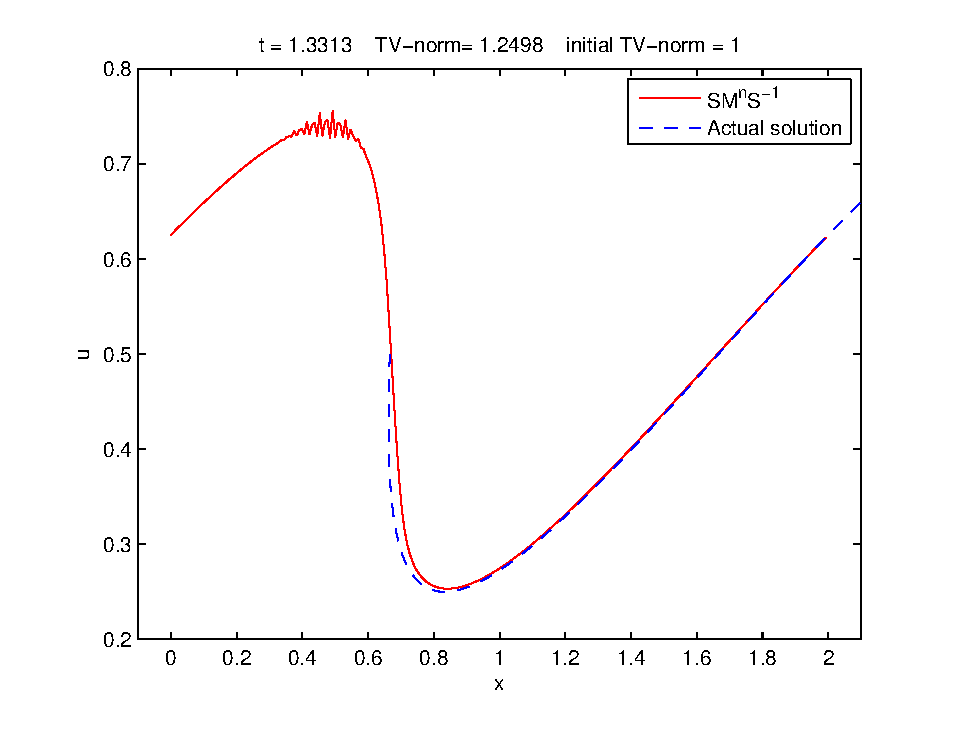
\includegraphics[width=0.5\textwidth]{Pictures/burgers_cont_no_tvd}}
    \caption{Solution of Burgers' equation with continuous initial data, using a 
    $TM^{n-2}R$ scheme, where $ M $ is SSPRK($10,4,2$). 
    The SSP coefficient is $\sspcoef =$.}
    \label{fig:burgers_cont}
\end{figure}

Burgers' equation was solved using an ESSPRK-scheme with time-step 
restriction $\Dt \leq \sigma{\Dt}_{FE}$, where $\sigma$ indicates the size 
of the time step. 
Figure \ref{fig:burgers_cont} shows that if $\sigma$ stays below the SSP 
coefficient of the method $M$, then no oscillations are observed. 
If this stability limit is violated, then oscillations appear. 
\yiannistodo{Elaborate more: Sharpness of SSP coefficient} 
We were able to determine when exactly the nonlinear stability is not 
satisfied by computing the the total-variation (TV) norm at each step of the 
computation process. 
This indicates that the ESSPRK-scheme inherits the time-step restriction 
from the SSP coefficient of the main method $M$.
\newline

We also consider the Burgers' equation with discontinuous data
\begin{equation}\label{eq:burgers_discont_IC}
    u(0,x)  = \left\{
                \begin{array}{ll}
                  1, & \hbox{$0.5 \leq x \leq 1.5$} \\
                  0, & \hbox{otherwise.}
                \end{array}
              \right.
\end{equation}
Figure~\ref{fig:burgers_discont} shows the result of solving the 
discontinuous problem using an ESSPRK-scheme, where $M$ is an 
SSPRK($4,4,3$) method. 
The scheme preservers monotonicity in the TV-norm since the starting 
method $R$ is SSP. 
This is illustrated in Figure~\ref{fig:burgers_starting_method} in which 
the solution plotted after one step using methods $R$ and $S$ as the 
starting procedures.

\begin{figure}[t!]
    \centering
    \subfloat[$\sigma = $]{\label{fig:burgers_discont_a}
      \includegraphics[width=0.5\textwidth]{Pictures/burgers_discont_tvd.eps}}
    \subfloat[$\sigma = $]{\label{fig:burgers_discont_a}
      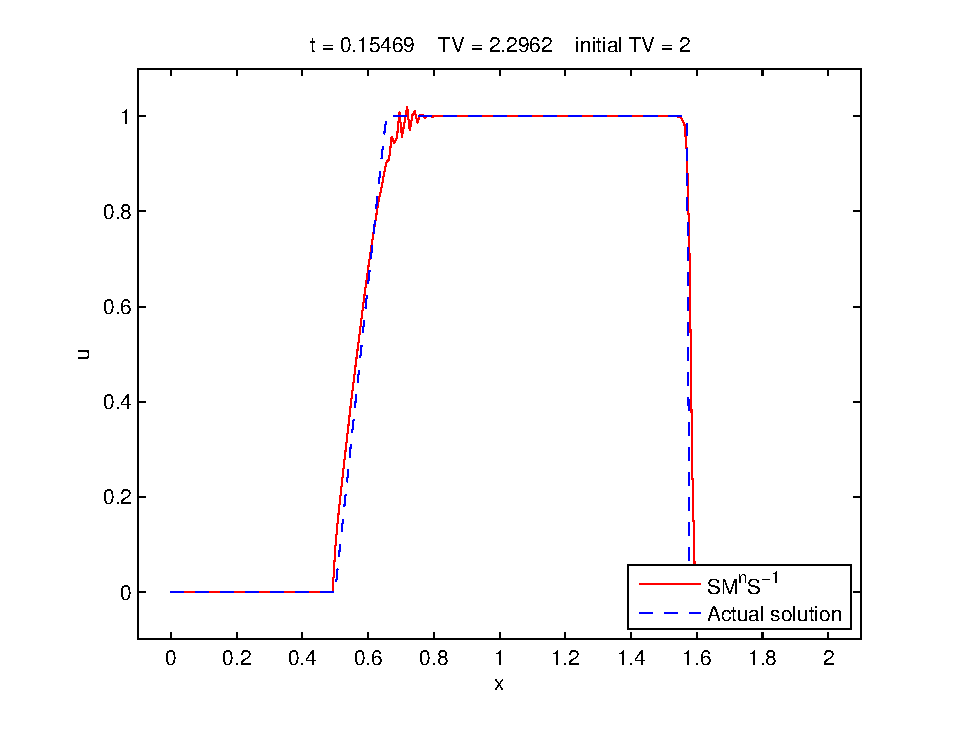
\includegraphics[width=0.5\textwidth]{Pictures/burgers_discont_no_tvd.eps}}
    \caption{Solution of Burgers' equation with discontinuous initial data, using a 
    $TM^{n-2}R$ scheme, where $M$ is SSPRK($4,4,3$) method. 
    The SSP coefficient is $ \sspcoef = $.}
    \label{fig:burgers_discont}
\end{figure}

\begin{figure}[t!]
    \centering
    \subfloat[]{\label{fig:burgers_starting_method_R}
      \includegraphics[width=0.5\textwidth]{Pictures/burgers_discont_tvd.eps}}
    \subfloat[]{\label{fig:burgers_starting_method_S}
      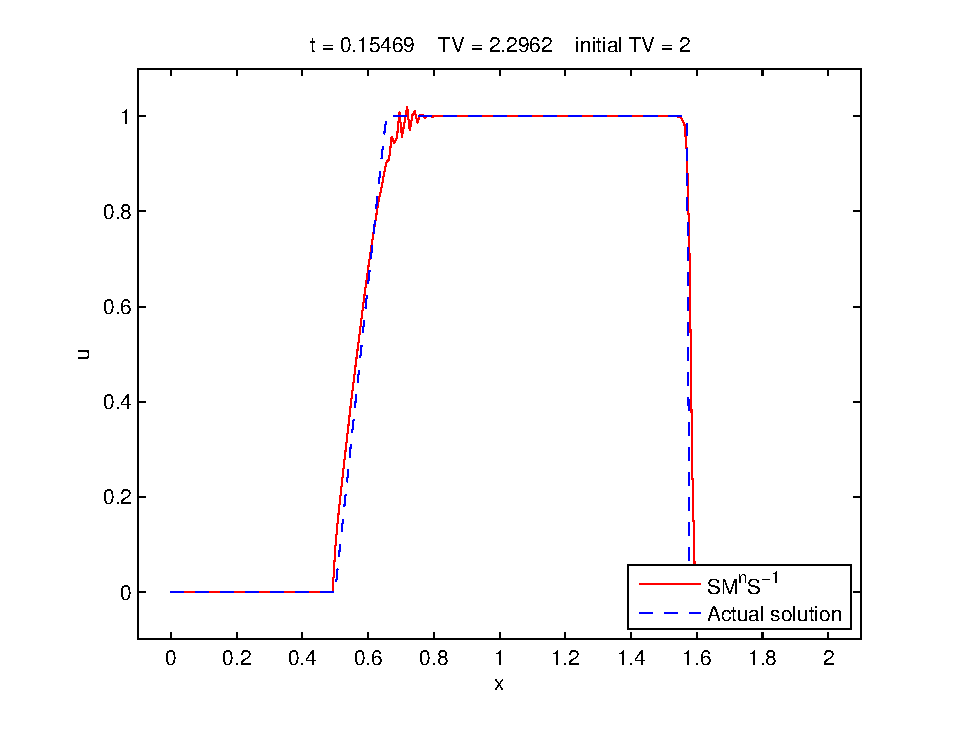
\includegraphics[width=0.5\textwidth]{Pictures/burgers_discont_no_tvd.eps}}
    \caption{Solution of Burgers' equation with discontinuous initial data 
    after one step, using a $TM^{n-2}R$ scheme, where $M$ is an 
    SSPRK($5,4,2$) method. The solution is advanced one step by using (a) $R$ and 
    (b) $S$}
    \label{fig:burgers_starting_method}
\end{figure}

